\section{Objetivos}
\begin{itemize}
    \item Determinar las líneas de campo de diferentes imanes para visualizar y entender la influencia magnética que ejercen en su entorno.
    \item Desarrollar una comprensión de la medición del campo magnético, familiarizándose con sus unidades y métodos de medición en diferentes configuraciones.
    \item Diferenciar entre diversos tipos de imanes y explorar sus aplicaciones prácticas en tecnología y dispositivos cotidianos.
    \item Determinar experimentalmente el campo magnético terrestre en el laboratorio, aplicando conceptos teóricos y técnicas de medición directa.
\end{itemize}

\section{Marco Teórico}
Los imanes son fundamentales en numerosas aplicaciones tecnológicas, desde la generación de electricidad hasta el almacenamiento de datos. Estos objetos ejercen fuerzas sobre materiales ferromagnéticos y otros imanes, un fenómeno que se debe a sus campos magnéticos, los cuales son regiones espaciales influenciadas por las propiedades magnéticas de los imanes.

\subsection{Naturaleza de los Imanes}
Descubiertos históricamente en la forma de magnetita, los imanes permanentes como el hierro, el níquel y el cobalto, poseen polos norte y sur, donde el campo magnético es más intenso. La interacción entre estos polos sigue reglas específicas: polos iguales se repelen y polos opuestos se atraen. Esta propiedad es invariable; al dividir un imán, cada fragmento siempre contará con ambos polos.

\subsection{Campo Magnético Terrestre}
La Tierra misma es un imán gigante con un campo magnético que interactúa con los imanes locales y afecta a brújulas y otros dispositivos de navegación. Este laboratorio busca medir y entender tanto los campos magnéticos generados por imanes artificiales como el campo magnético terrestre.

\subsection{Campo Magnético de las Bobinas de Helmholtz}
Se utilizarán bobinas de Helmholtz para generar un campo magnético controlable y medir su interacción con el campo terrestre. Estas bobinas permiten crear un campo magnético homogéneo que se puede ajustar mediante cambios en la corriente eléctrica suministrada, lo que es crucial para estudios precisos de campos magnéticos.

La comprensión y aplicación de estos conceptos permite no solo apreciar cómo funcionan los dispositivos basados en el magnetismo, sino también desarrollar nuevas aplicaciones y mejorar las tecnologías existentes.

\section{Análisis y discusión: Montaje 1 Imanes}

\subsection{Determine las líneas de campo con imanes}
\textbf{Con las limaduras de hierro determine las líneas de campo de los diferentes imanes,
describa lo que observa}
Al esparcir limaduras de hierro sobre una lámina de vidrio con diferentes imanes dispuestos debajo, se pudo observar claramente la forma y dirección de las líneas de campo magnético. En cada caso, las limaduras se alinearon formando patrones que delinean las líneas de campo emanadas desde los polos de los imanes.

\begin{figure}[H]
  \centering
  \begin{minipage}{0.45\textwidth}
    \centering
    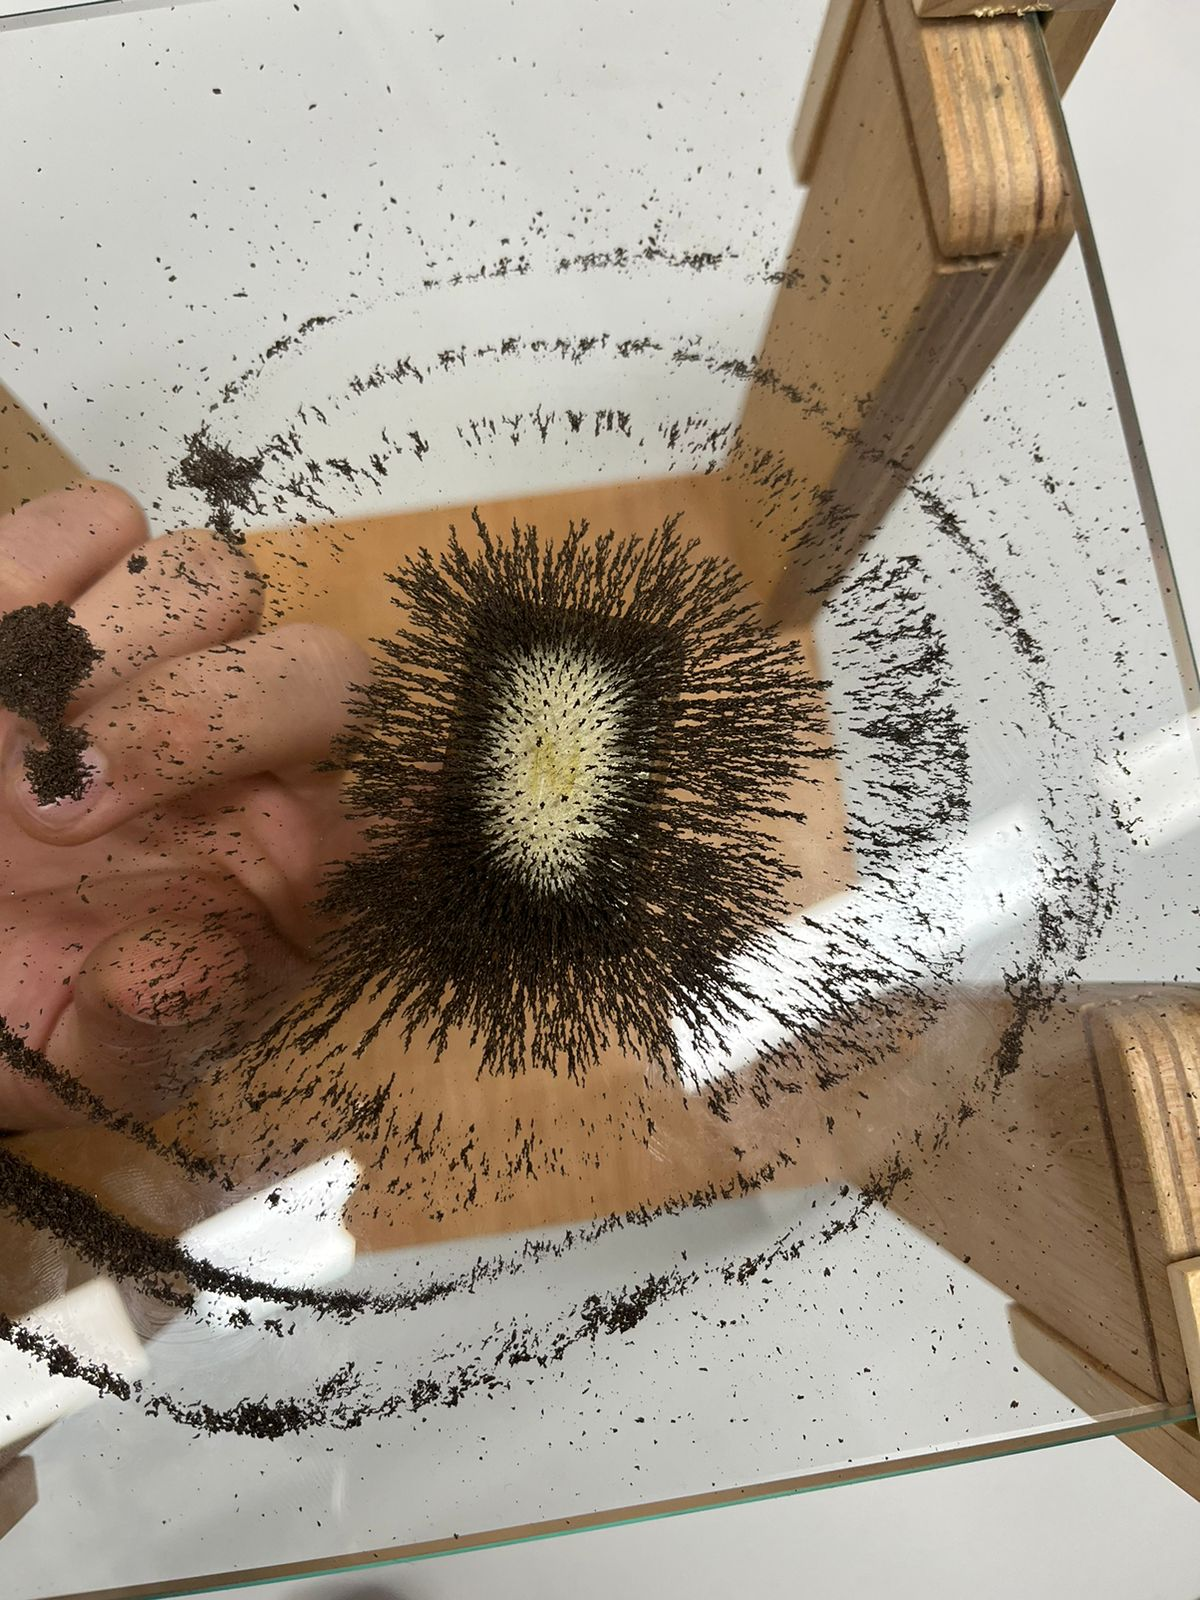
\includegraphics[width=\textwidth]{Figures/1. Content/LimadurasHierro3.jpeg}
    \captionof{figure}{Líneas de campo de limaduras de hierro con imán 1}
    \label{fig: Limadura de Hierro 3}
  \end{minipage}
  \hfill
  \begin{minipage}{0.45\textwidth}
    \centering
    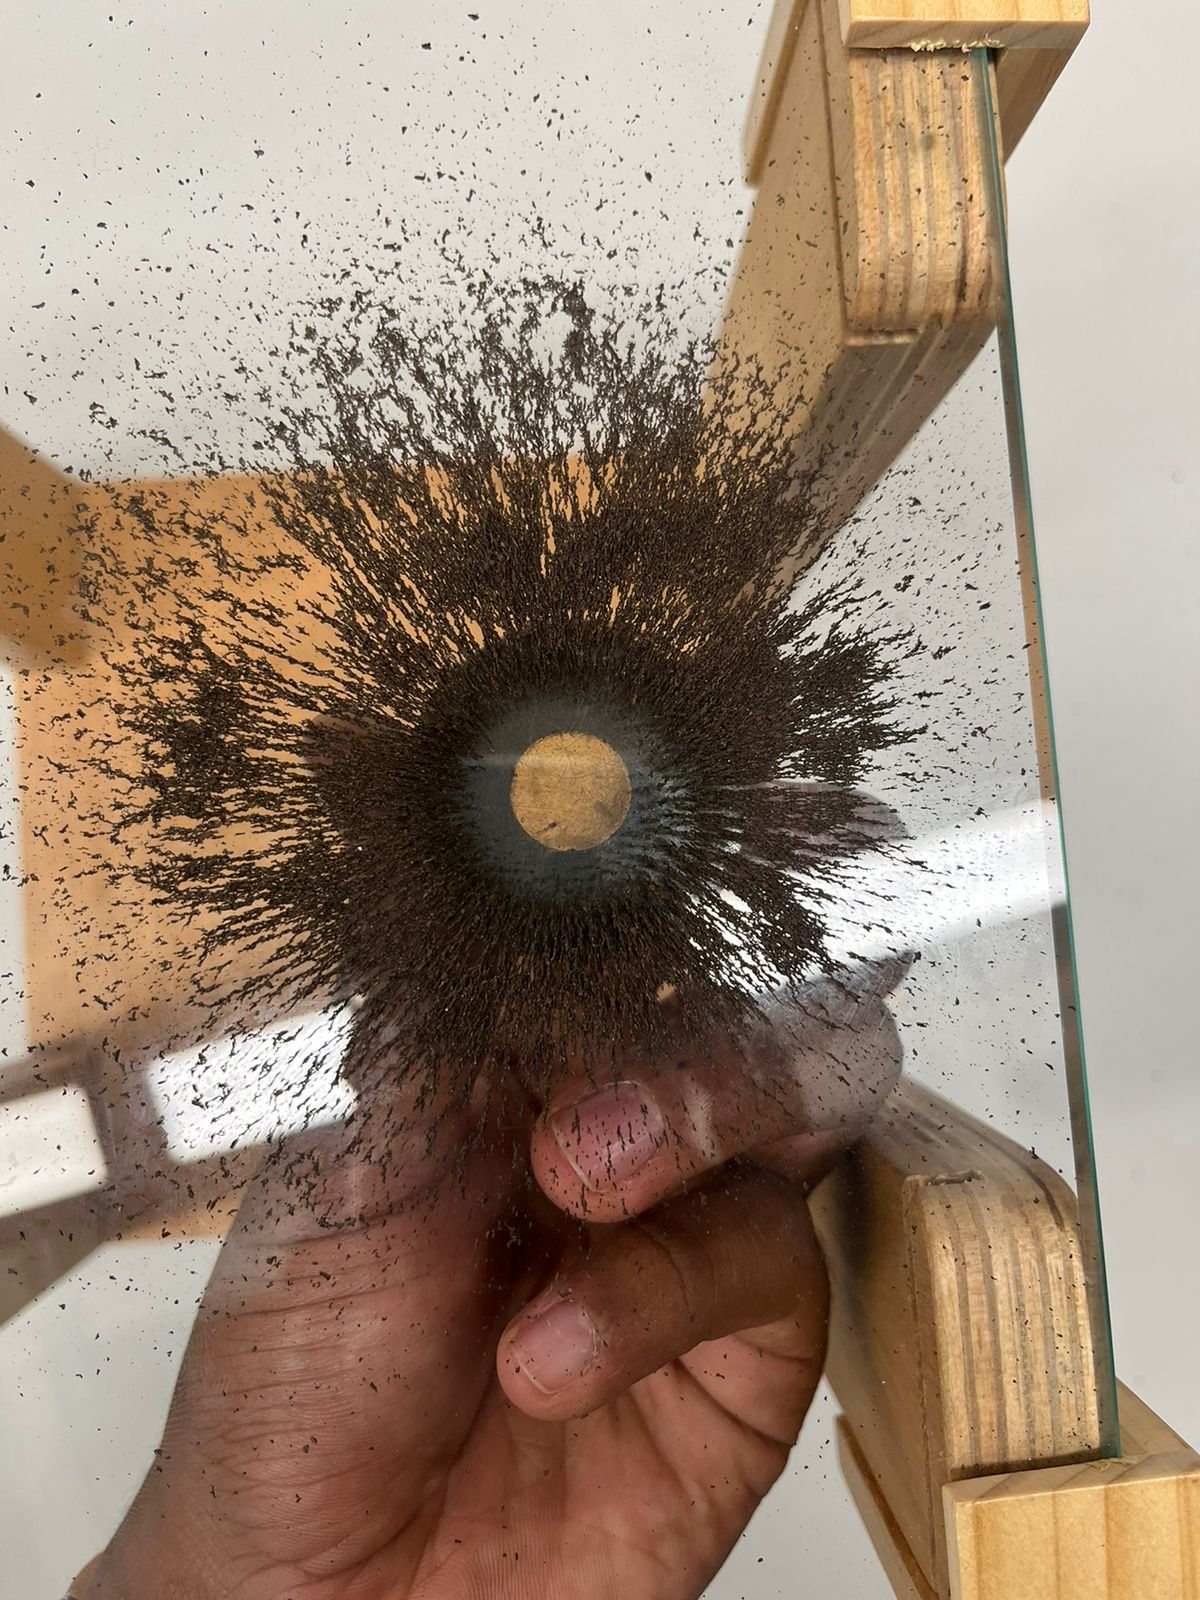
\includegraphics[width=\textwidth]{Figures/1. Content/LimadurasHierro1.jpeg}
    \captionof{figure}{Líneas de campo de limaduras de hierro con imán 2}
    \label{fig: Limadura de Hierro 1}
  \end{minipage}
  \hfill
  \begin{minipage}{0.45\textwidth}
    \centering
    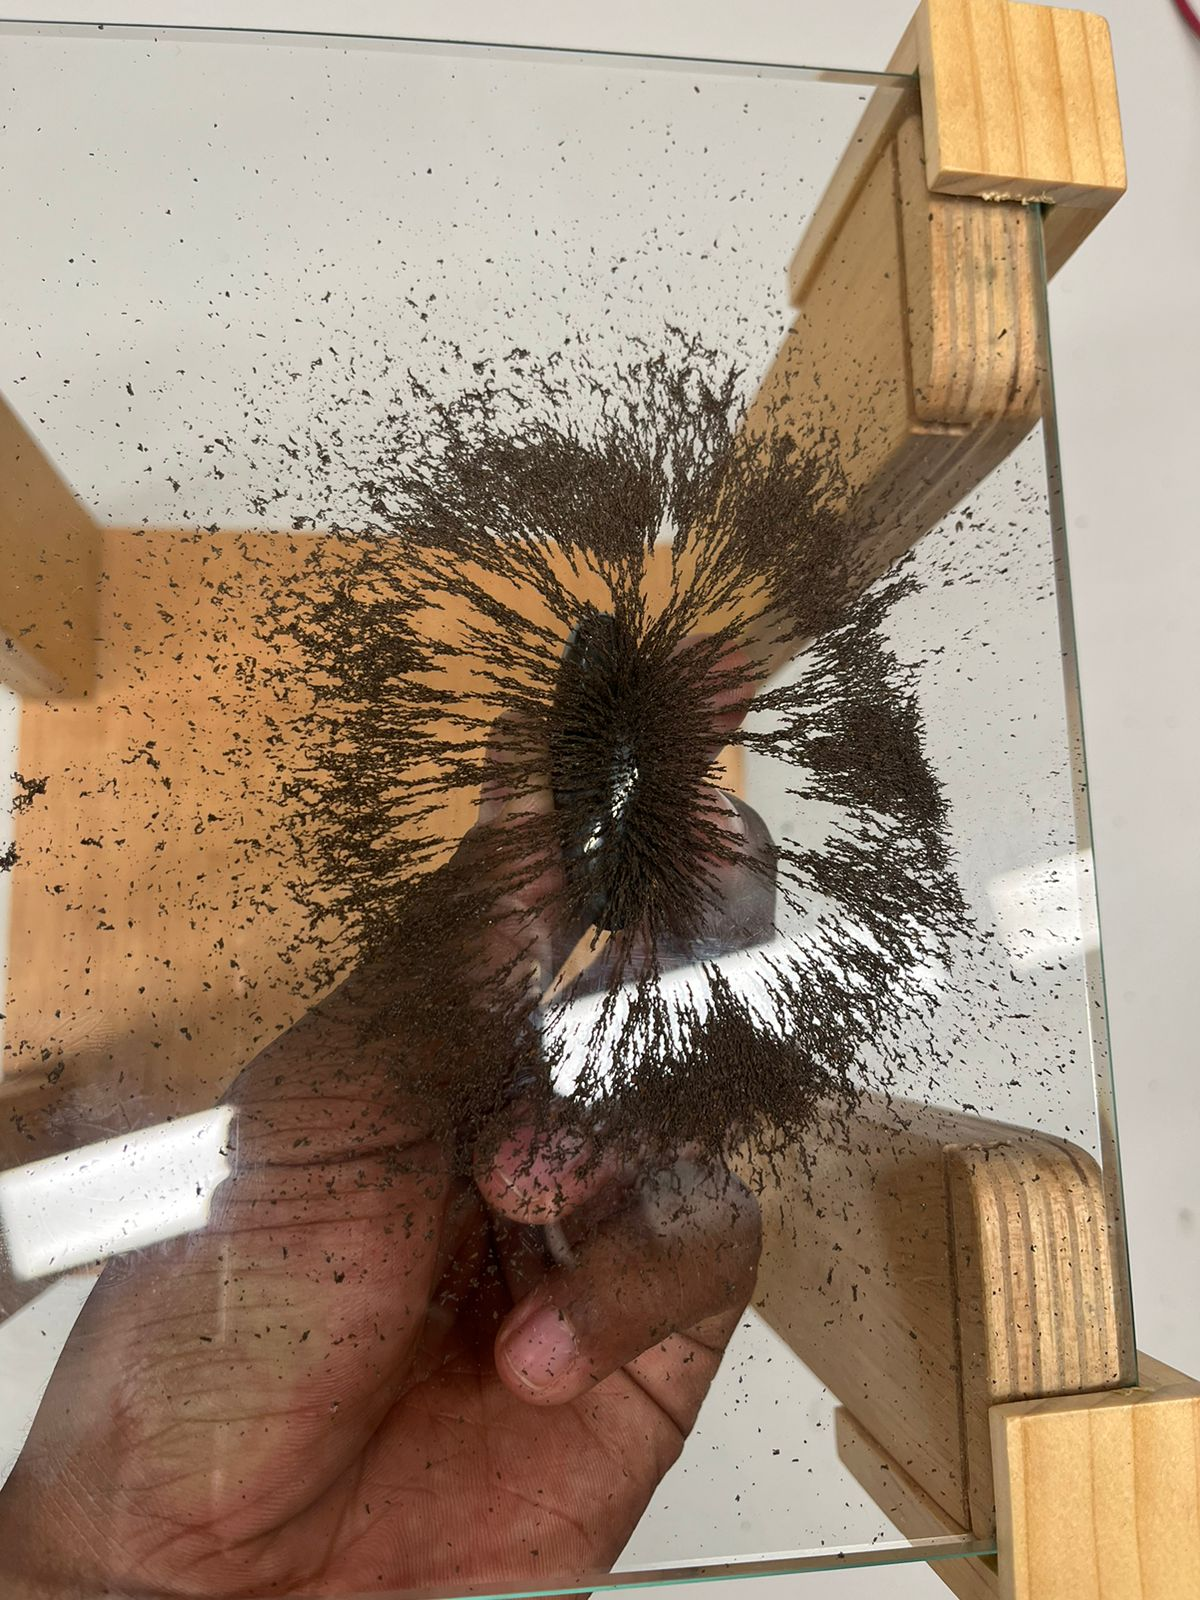
\includegraphics[width=\textwidth]{Figures/1. Content/LimadurasHierro2.jpeg}
    \captionof{figure}{Líneas de campo de limaduras de hierro con imán 3}
    \label{fig: Limadura de Hierro 2}
  \end{minipage}
  \hfill

\end{figure}

\begin{itemize}
  \item \textbf{Imán 1:} Las limaduras se organizaron en un patrón radial alrededor del imán, mostrando un punto central desde donde parece emanar el campo. Esto sugiere un imán con un solo polo dominante visible o un disco magnético con un campo concentrado en el centro.

  \item \textbf{Imán 2:} El patrón formado por las limaduras indica un campo magnético clásico de un dipolo, con líneas que emergen desde un extremo del imán y reingresan en el otro. Esto es típico de un imán de barra, donde las líneas de campo se curvan desde el polo norte hacia el polo sur.

  \item \textbf{Imán 3:} Similar al segundo imán, pero con líneas de campo que se extienden más ampliamente alrededor de los polos, indicando posiblemente un campo más fuerte o un imán de mayor tamaño. Las líneas son más dispersas, lo que sugiere una interacción más fuerte con el entorno circundante.
\end{itemize}

Estas observaciones permiten visualizar y comprender la forma en que el campo magnético interactúa con materiales ferromagnéticos y cómo se manifiesta el flujo magnético en el espacio alrededor de diferentes tipos de imanes.


\subsection{Encontrar los polos de los imanes}
\textbf{Con dos imanes, encuentre los polos norte y sur de cada uno de ellos.
Describa lo que sucede.}

\begin{figure}[H]
  \centering
  \begin{minipage}{0.3\textwidth}
    \centering
    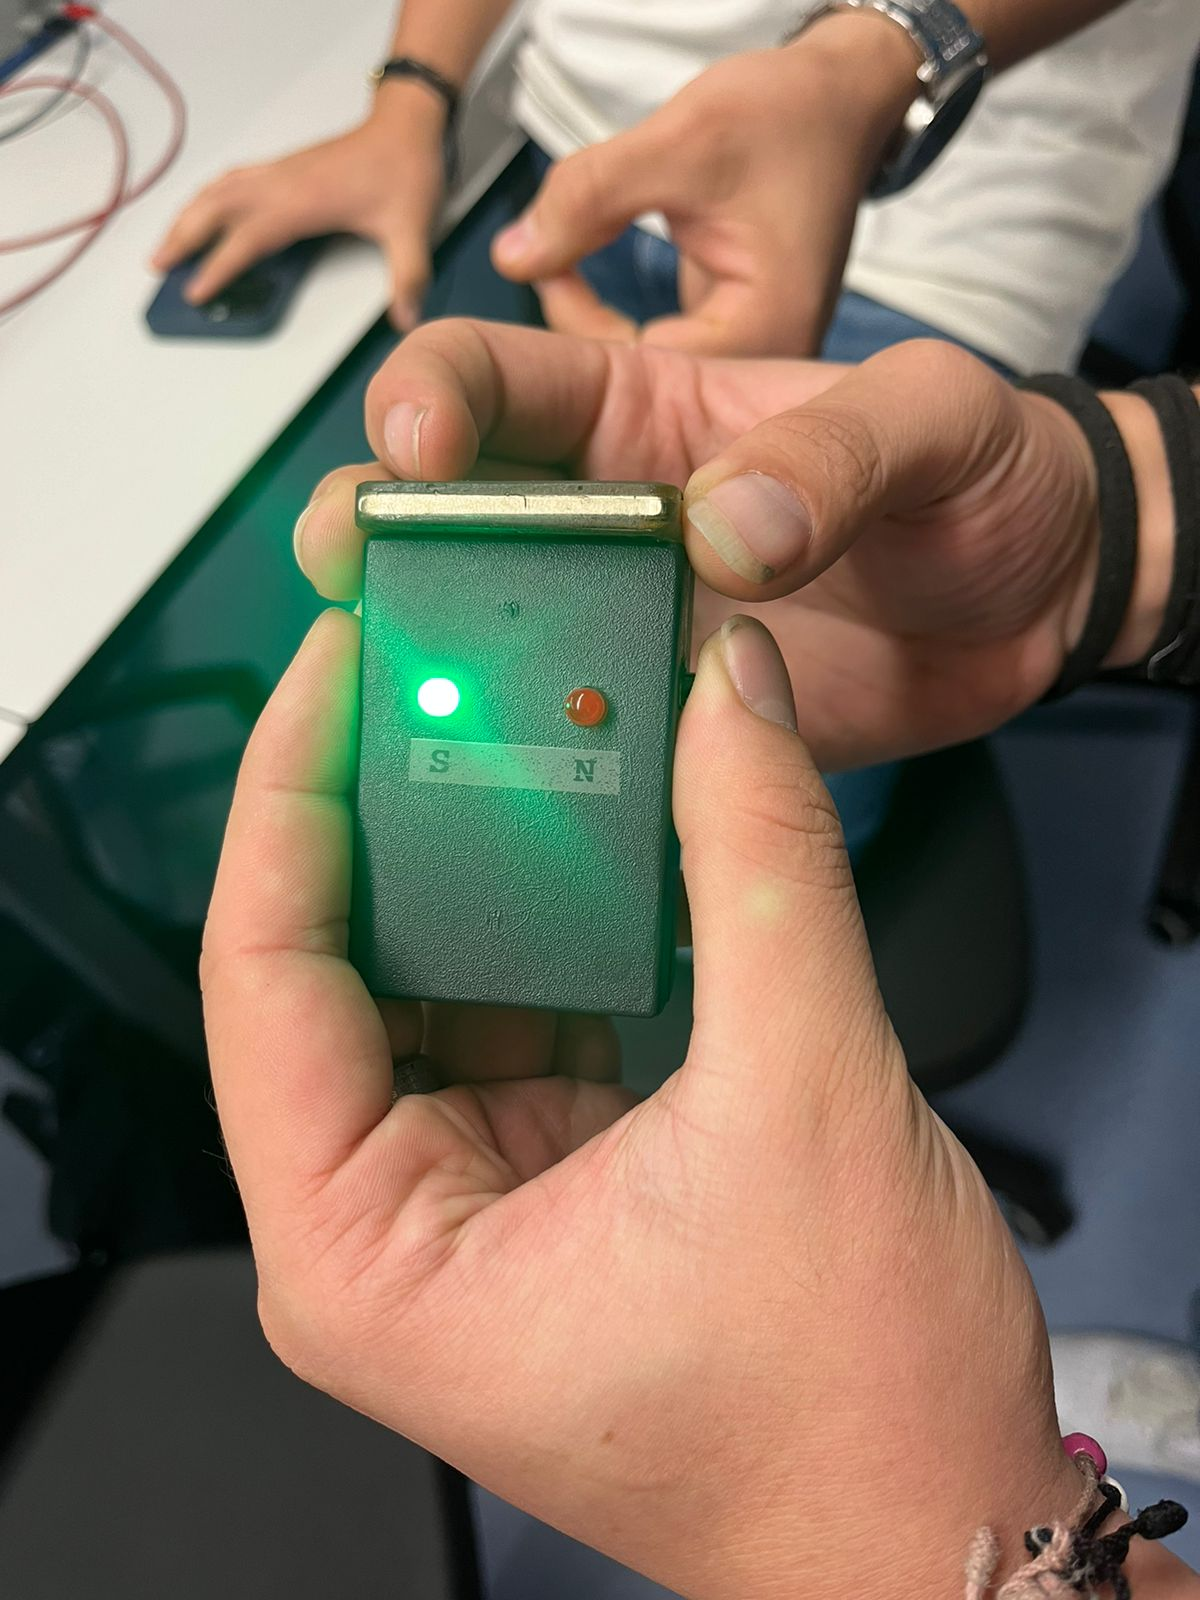
\includegraphics[width=\textwidth]{Figures/1. Content/BuscarPolaridad5.jpeg}
    \captionof{figure}{Polaridad Positiva del Imán 1}
    \label{fig: Polaridad Positiva del Iman 1}
  \end{minipage}
  \hfill
  \begin{minipage}{0.3\textwidth}
    \centering
    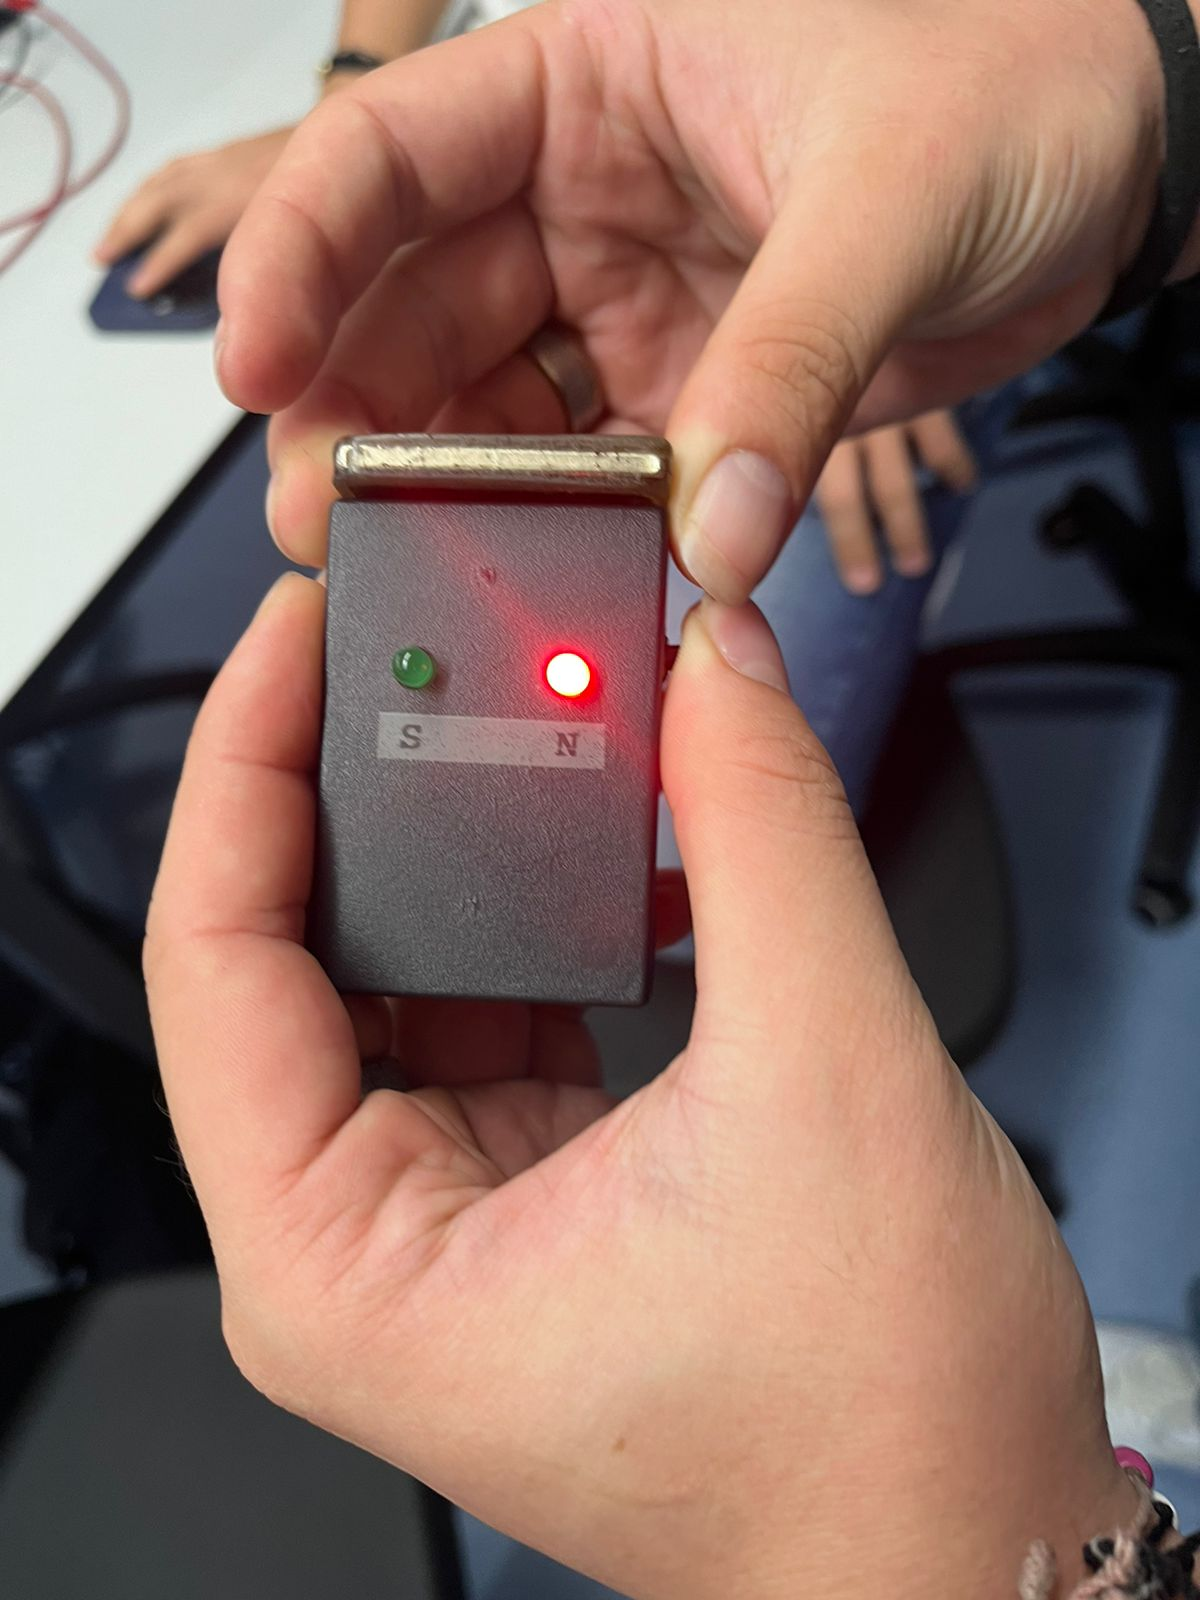
\includegraphics[width=\textwidth]{Figures/1. Content/BuscarPolaridad6.jpeg}
    \captionof{figure}{Polaridad Negativa del Imán 1}
    \label{fig: Polaridad Negativa del Iman 1}
  \end{minipage}
  \hfill
  \begin{minipage}{0.3\textwidth}
    \centering
    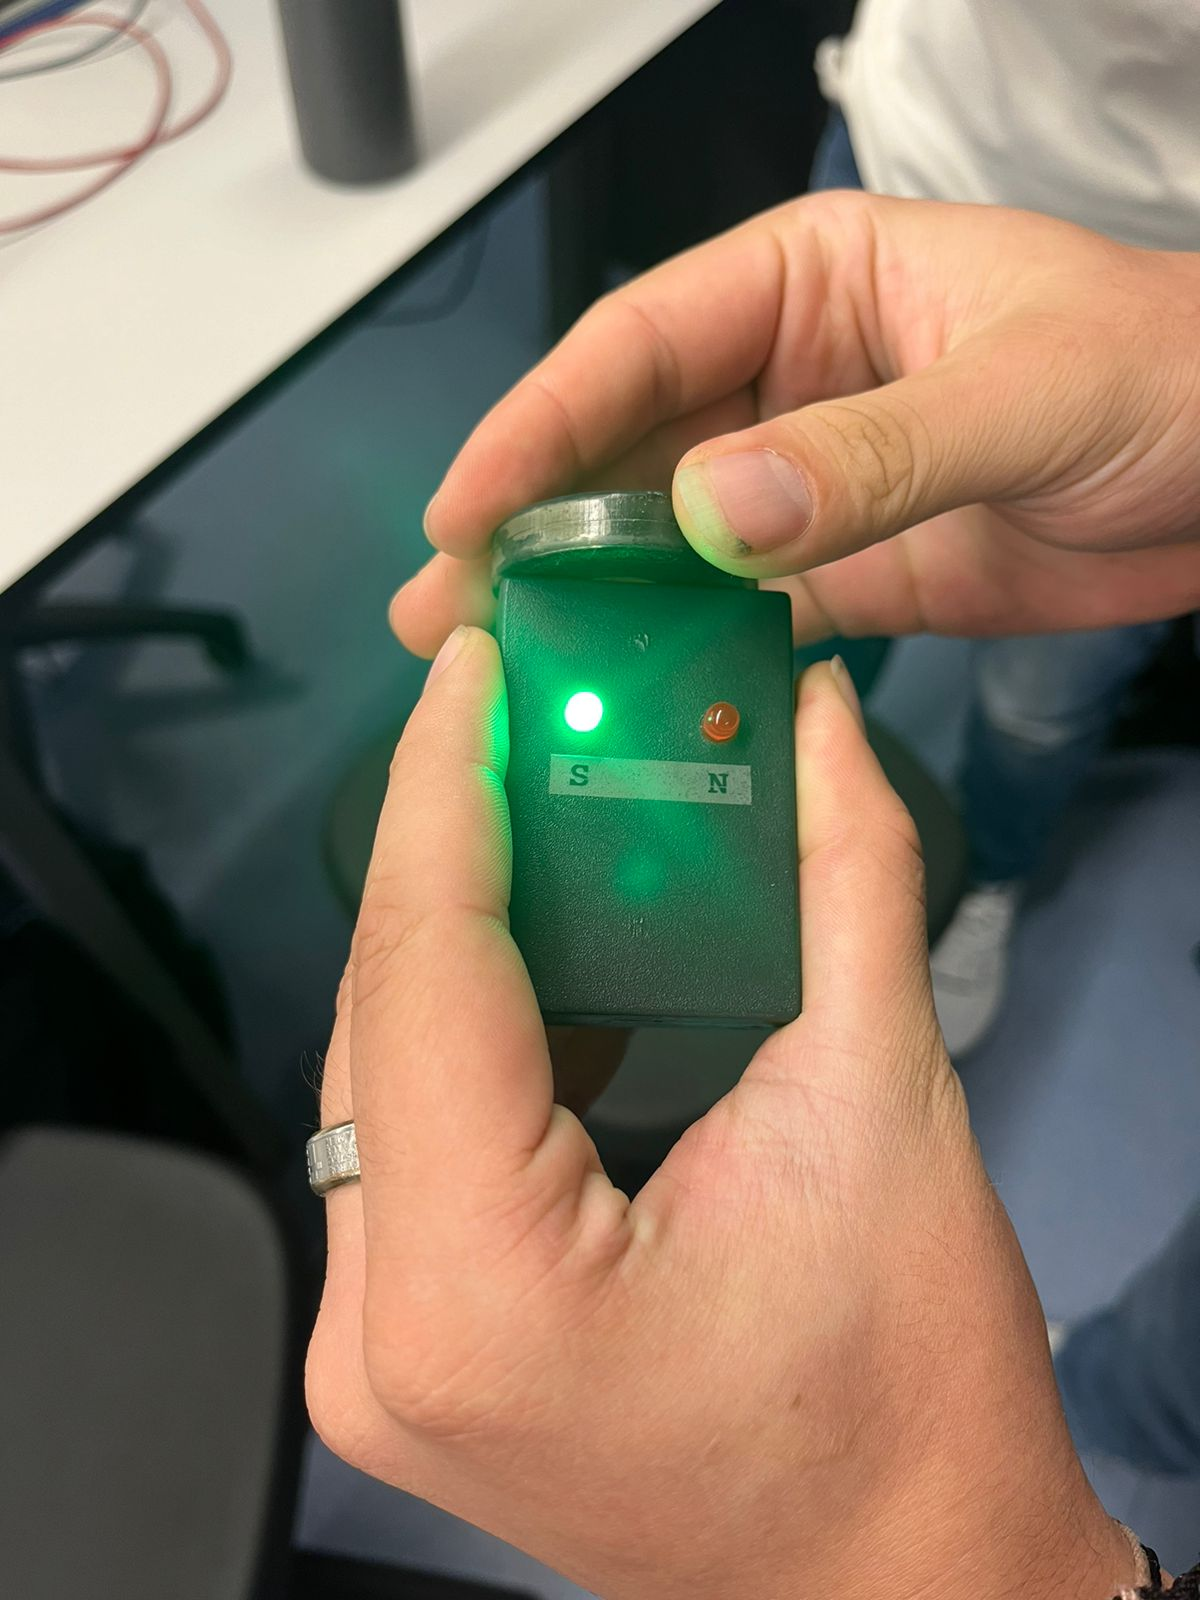
\includegraphics[width=\textwidth]{Figures/1. Content/BuscarPolaridad1.jpeg}
    \captionof{figure}{Polaridad Positiva del Imán 2}
    \label{fig: Polaridad Positiva del Iman 2}
  \end{minipage}
  \hfill
  \begin{minipage}{0.3\textwidth}
    \centering
    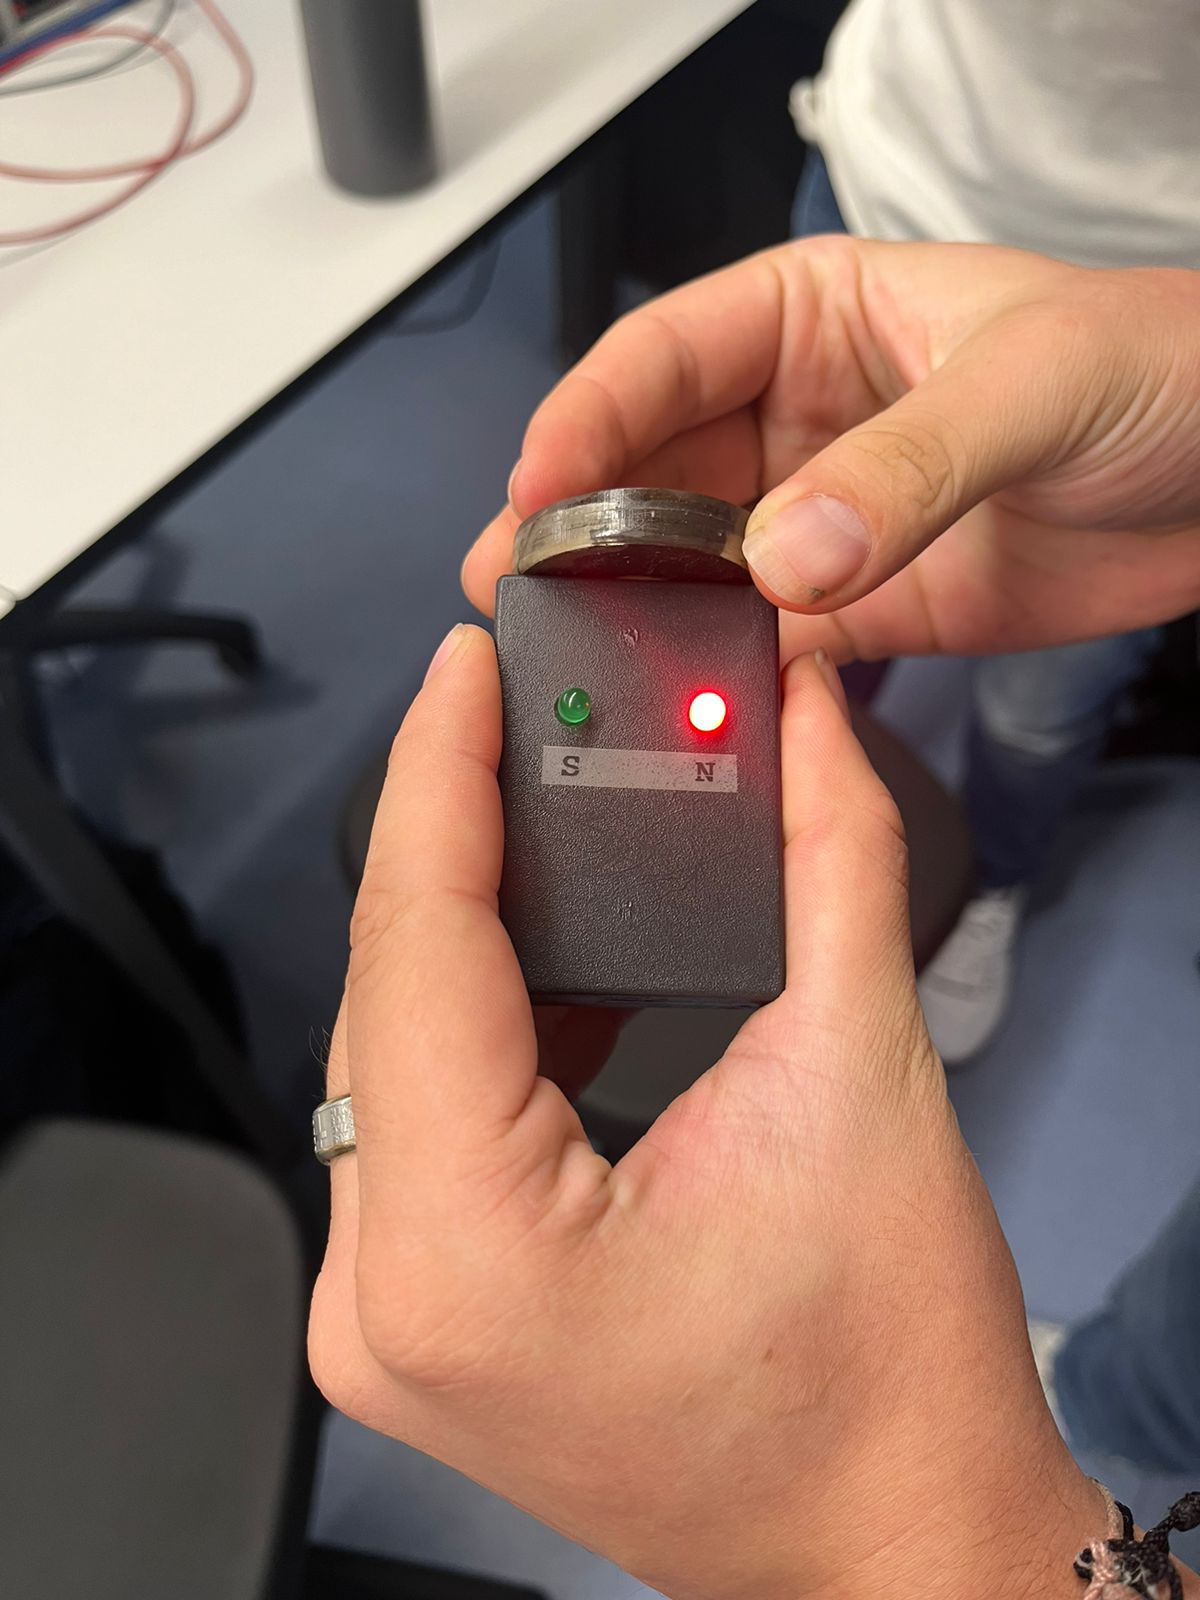
\includegraphics[width=\textwidth]{Figures/1. Content/BuscarPolaridad2.jpeg}
    \captionof{figure}{Polaridad Negativa del Imán 2}
    \label{fig: Polaridad Negativa del Iman 2}
  \end{minipage}
  \hfill
  \begin{minipage}{0.3\textwidth}
    \centering
    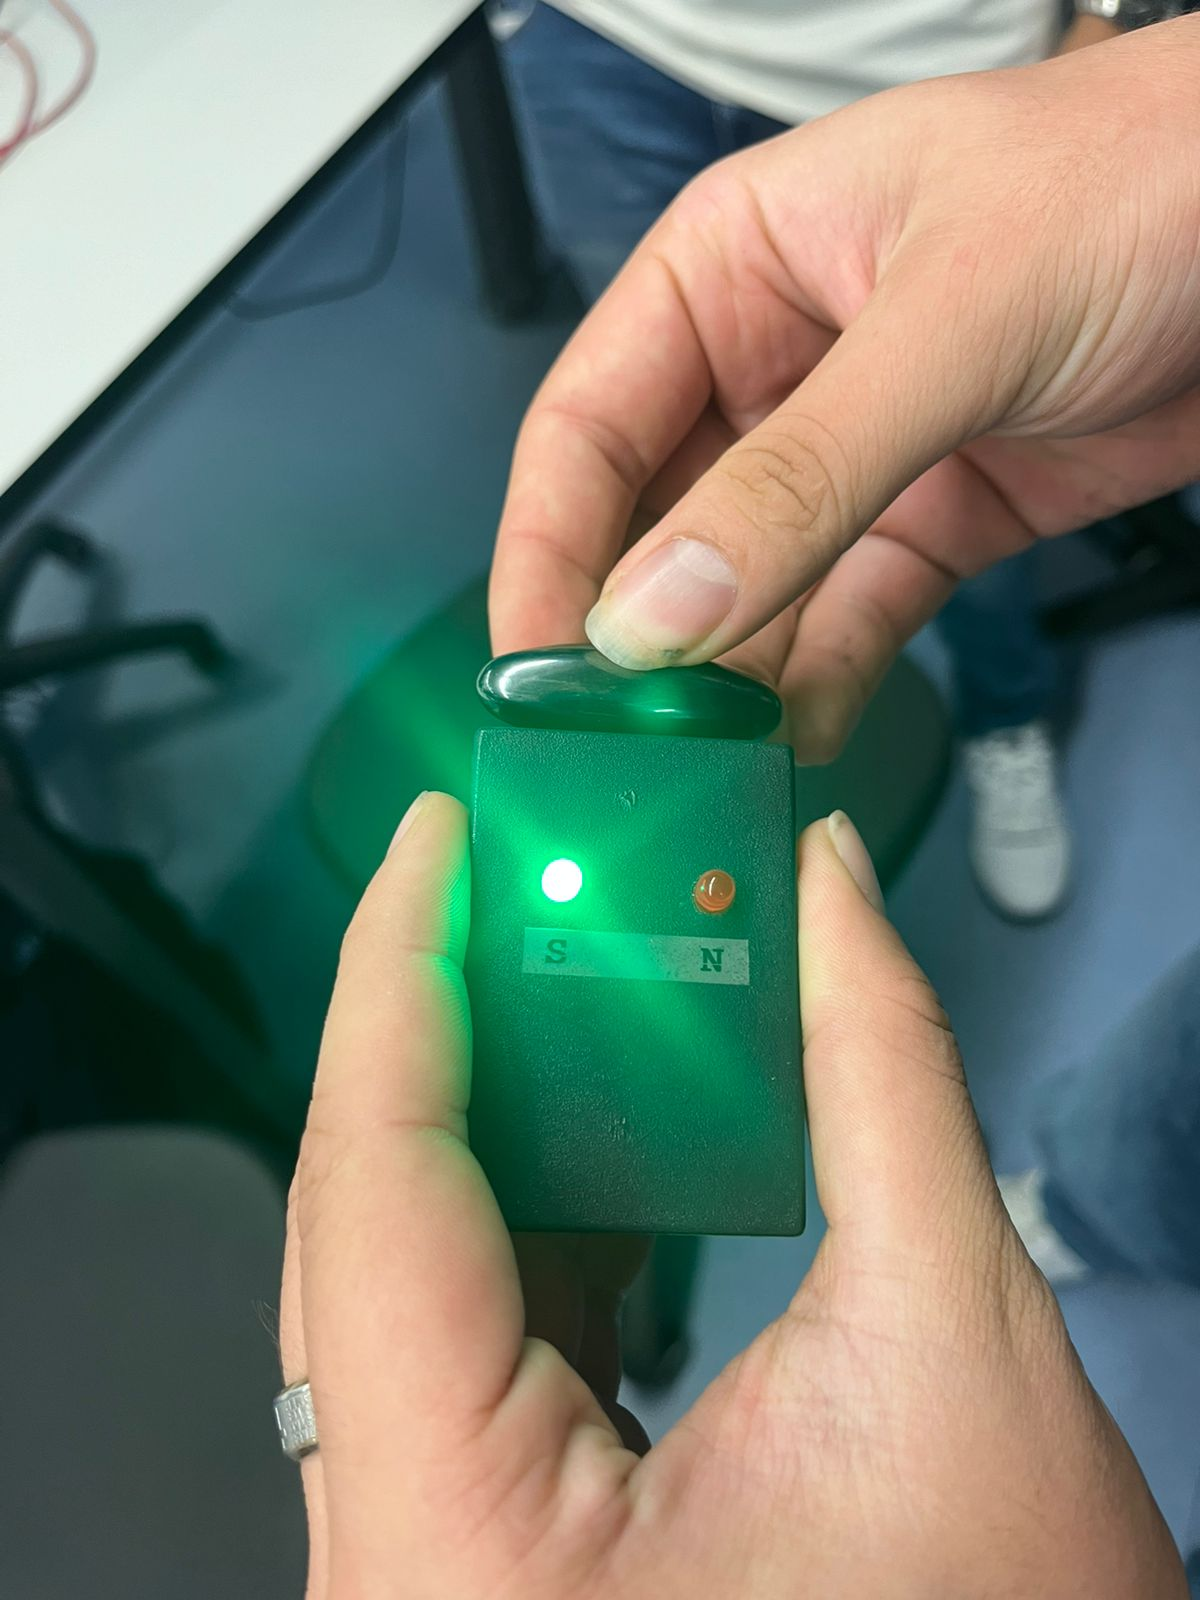
\includegraphics[width=\textwidth]{Figures/1. Content/BuscarPolaridad3.jpeg}
    \captionof{figure}{Polaridad Positiva del Imán 3}
    \label{fig: Polaridad Positiva del Iman 3}
  \end{minipage}
  \hfill
  \begin{minipage}{0.3\textwidth}
    \centering
    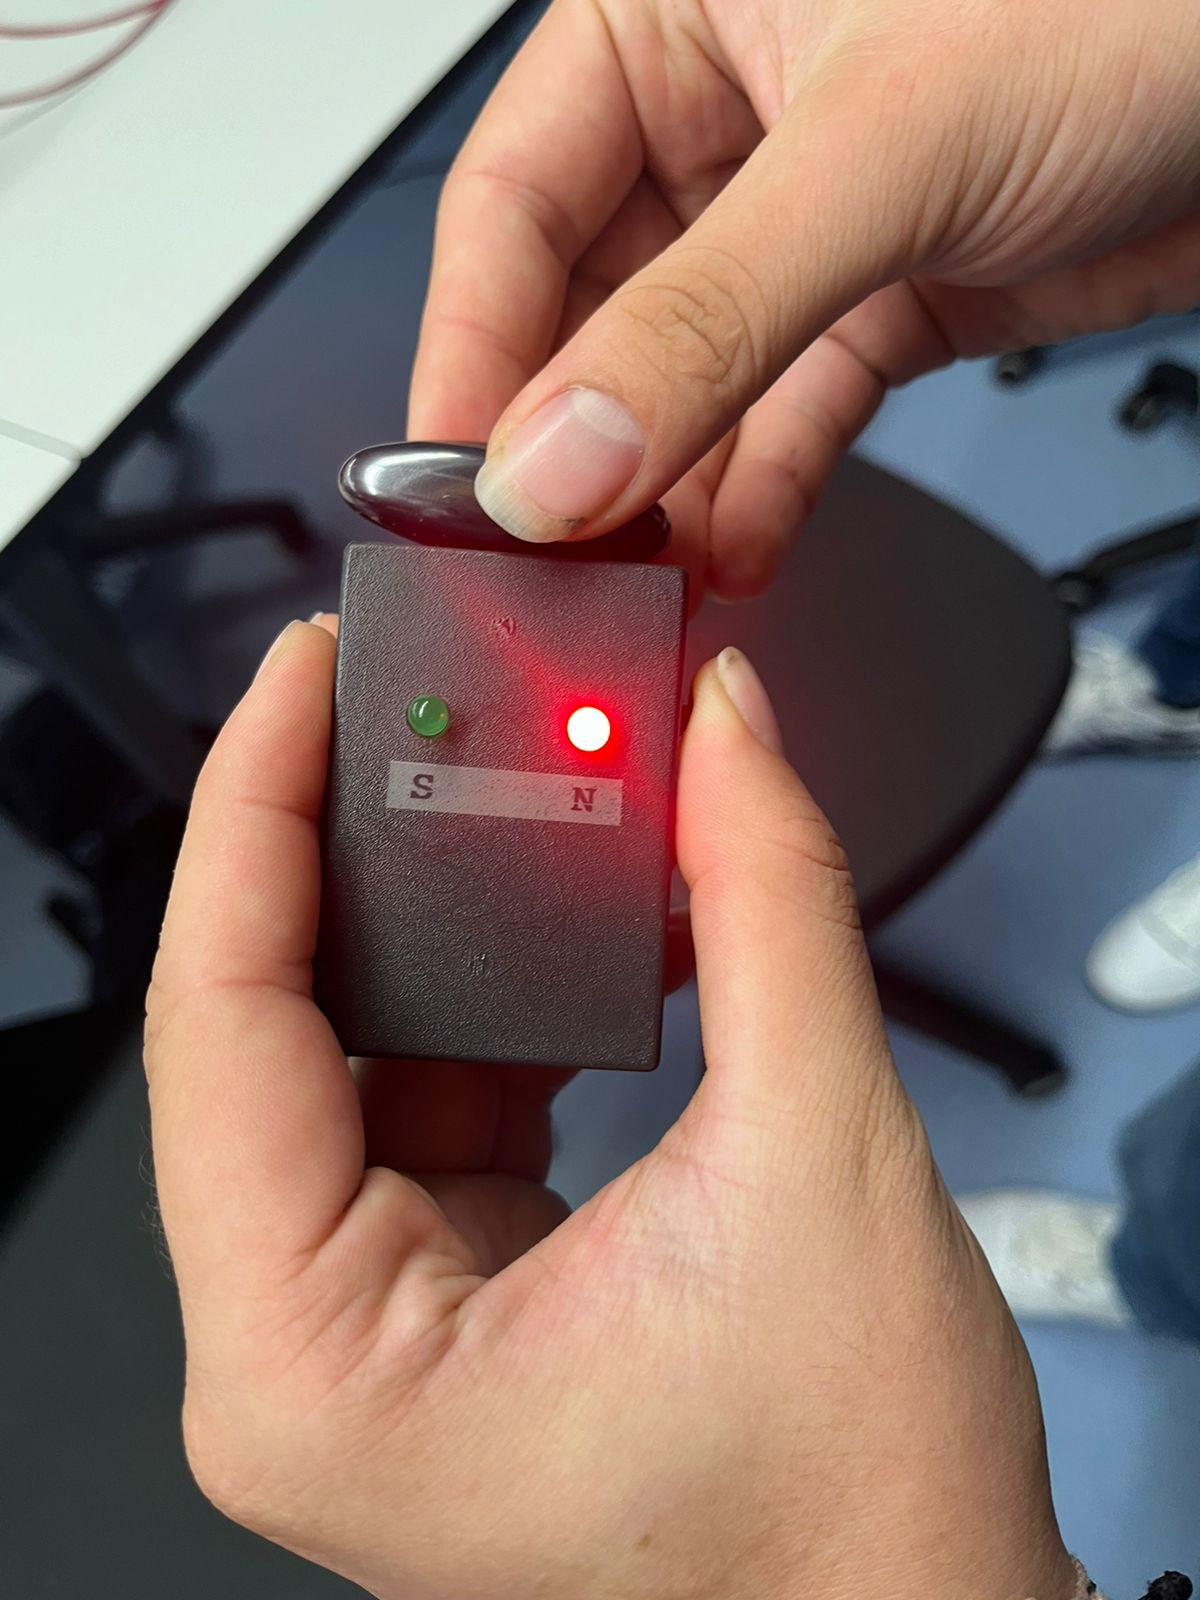
\includegraphics[width=\textwidth]{Figures/1. Content/BuscarPolaridad4.jpeg}
    \captionof{figure}{Polaridad Negativa del Imán 3}
    \label{fig: Polaridad Negativa del Iman 3}
  \end{minipage}
  \hfill
\end{figure}

Para identificar los polos de los imanes, se utilizó un dispositivo detector de polaridad que indica mediante luces LED el tipo de polo que se está examinando: verde para el polo norte y rojo para el polo sur. Al aproximarse los imanes uno hacia el otro, observamos las siguientes reacciones:

\begin{itemize}
    \item Cuando los polos opuestos de dos imanes se acercan (norte con sur), las luces indicadoras muestran colores diferentes en cada imán (uno verde y el otro rojo), lo cual indica una atracción. Este fenómeno es consistente con la ley de magnetismo que dicta que polos opuestos se atraen.
    \item Al enfrentar los mismos polos (norte con norte o sur con sur), las luces muestran el mismo color en ambos imanes, indicando que estamos frente a polos iguales. En esta configuración, se observa una repulsión clara entre los imanes, donde cada uno intenta alejarse del otro, validando la ley que polos iguales se repelen.
\end{itemize}

Estas observaciones no solo confirmaron la funcionalidad del detector de polaridad, sino que también proporcionaron una visualización directa e interactiva de las interacciones fundamentales entre los campos magnéticos de los imanes.


\subsection{Comprobación de Interacciones Magnéticas}
\textbf{Para dos imanes compruebe que polos magnéticos del mismo tipo se repelen y polos magnéticos de distinto tipo se atraen. Para las siguientes situaciones, observe las posiciones en donde la atracción es máxima y las posiciones en donde la repulsión es máxima. Igualmente, se trata de visualizar el campo magnético con limaduras de hierro.}

En esta serie de experimentos, utilizamos dos imanes y limaduras de hierro para visualizar las líneas de campo magnético y verificar las interacciones entre diferentes configuraciones de polos:

\begin{enumerate}
    \item \textbf{Un imán solo:} Con un solo imán bajo una hoja de vidrio espolvoreada con limaduras de hierro, observamos cómo las limaduras se alinean a lo largo de las líneas del campo magnético, emanando del polo norte hacia el polo sur del imán, creando un patrón conocido de campo magnético.

    \item \textbf{Dos imanes con polos idénticos enfrentados:} Al enfrentar los polos norte con norte o sur con sur, las limaduras de hierro revelan un campo donde las líneas intentan alejarse una de la otra, indicando repulsión. Esta configuración mostró un claro espacio vacío entre los polos enfrentados donde las limaduras se repelían, evidenciando la máxima repulsión.

    \item \textbf{Dos imanes con polos opuestos enfrentados:} Contrariamente, al alinear los polos opuestos (norte con sur), las limaduras formaron un puente directo entre los dos imanes, indicando una fuerte atracción. Las limaduras se alinearon densamente entre los dos polos, mostrando la zona de máxima atracción donde las líneas de campo se unen directamente.
\end{enumerate}

Estos experimentos no solo demostraron visualmente las fuerzas fundamentales de atracción y repulsión magnética, sino que también permitieron observar cómo el campo magnético se distorsiona y adapta según la configuración de los imanes.

\subsection{Medición del Campo Magnético y Determinación de la Fuerza Magnética}
Medimos el campo magnético a una distancia constante utilizando un teslámetro para tres diferentes imanes: un imán rectangular, un imán circular, y un imán en forma de Elipsoide. Las mediciones se realizaron a distancias incrementales desde la superficie del imán hasta 8 mm. Los resultados son los siguientes:

\begin{itemize}
    \item \textbf{Imán 1 (Rectangular)}: Este imán mostró los valores más altos de campo magnético, empezando en 33.1 mT en la superficie y disminuyendo hasta 4.6 mT a una distancia de 8 mm.
    \item \textbf{Imán 2 (Circular)}: Este imán comenzó con un campo de 11.6 mT en la superficie, reduciéndose a 1.6 mT a 8 mm.
    \item \textbf{Imán 3 (Elipsoide)}: El campo magnético comenzó en 14.7 mT y bajó a 1.9 mT a 8 mm de distancia.
\end{itemize}

Los gráficos de la variación del campo magnético en función de la distancia muestran que el \textbf{Imán 1 (Rectangular)} tiene la mayor fuerza magnética en todas las distancias medidas, seguido por el \textbf{Imán 3 (Elipsoide)} y luego el \textbf{Imán 2 (Circular)}. Esto se refleja también en los cálculos de potencia, donde el imán rectangular domina significativamente en términos de influencia magnética a corta distancia.

Estos resultados sugieren que la geometría del imán juega un papel crucial en su capacidad para mantener un campo magnético a mayores distancias, con el imán rectangular mostrando la mayor eficacia en retener su fuerza magnética comparado con las formas circular y esférica.

\subsection{Tabla de cada imán}
\textbf{De acuerdo con la geometría del teslámetro construya la siguiente tabla, midiendo
el campo magnético de tres imanes diferentes a diferentes distancias.}

\begin{figure}[H]
    \centering
    \begin{subfigure}[b]{\textwidth}
        \centering
        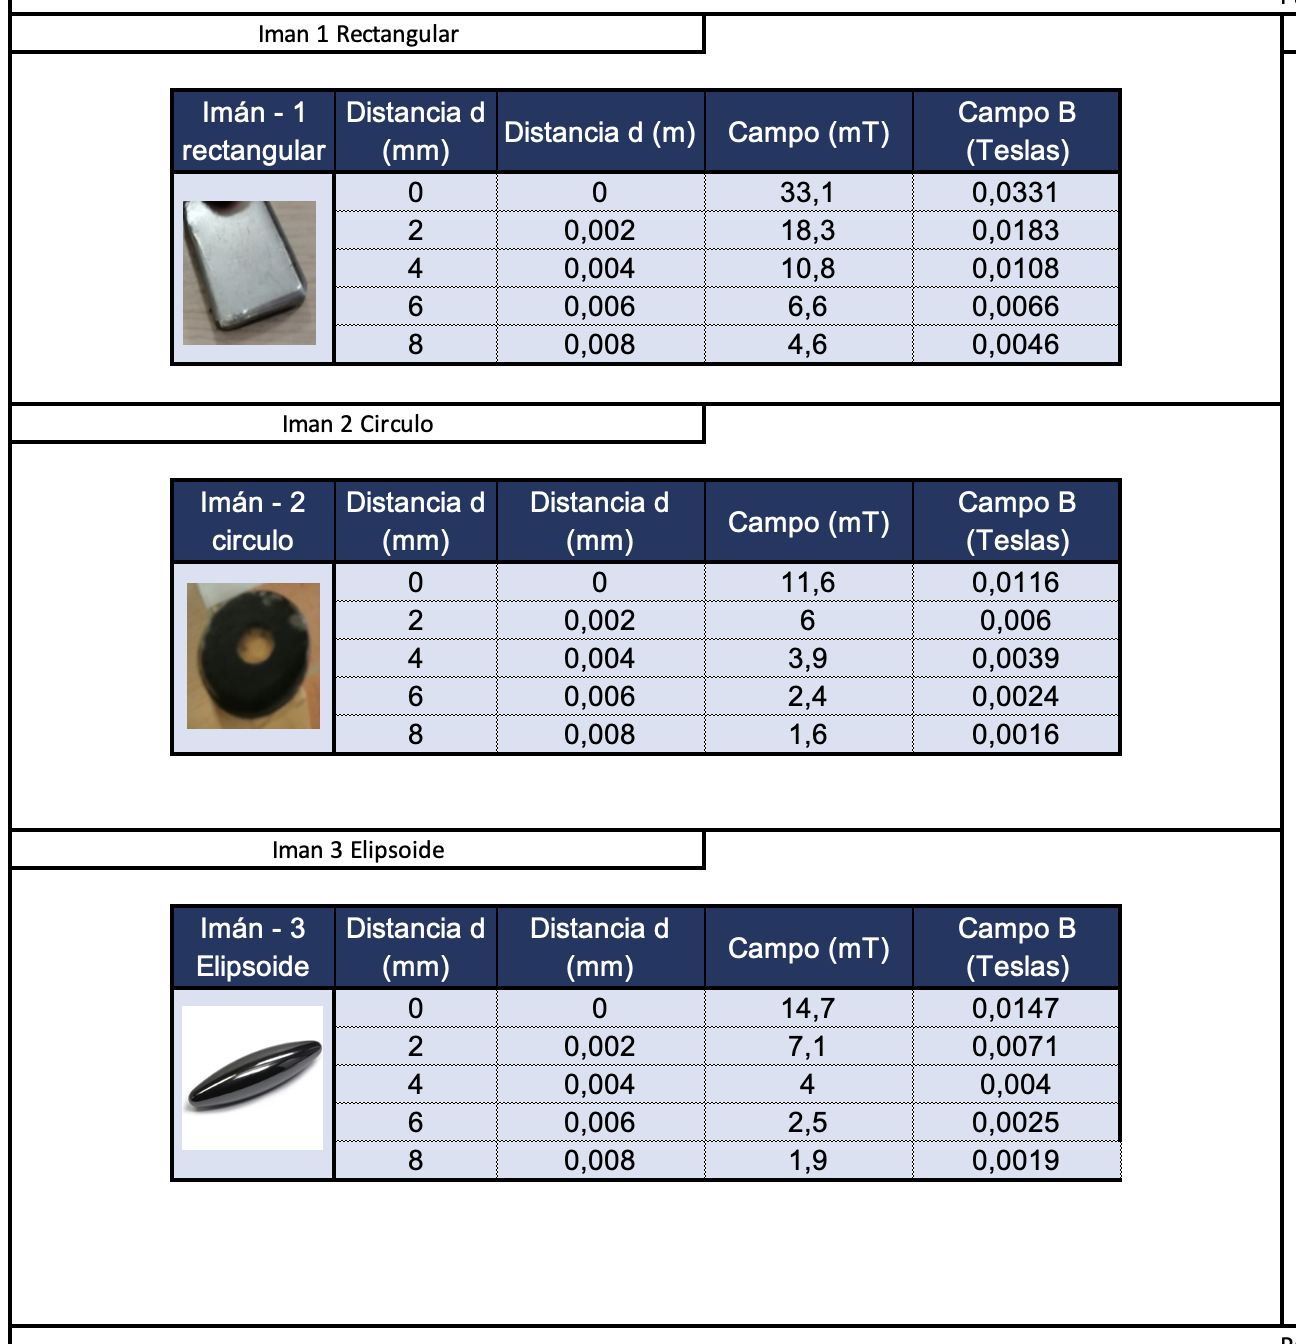
\includegraphics[width=\textwidth]{Figures/1. Content/TablaImanesTesla.png}
        \caption{Tabla de la medición de Teslas ($T$) por cada imán.}
        \label{fig: Tabla de geometria teslametro}
    \end{subfigure}
    \hfill
\end{figure}

\subsection{$B$ vs $d$}
\textbf{¿Cómo varía $B$ con $d$?}
El campo magnético $B$ disminuye con el aumento de la distancia $d$ desde la superficie del imán. Este comportamiento se puede observar claramente en los gráficos proporcionados, donde $B$ decrece de manera significativa a medida que $d$ aumenta. Esto es típico de los campos magnéticos, ya que siguen una ley de inversa del cuadrado, similar a otros tipos de campos en la física, como el campo eléctrico y gravitacional.

\subsection{Imán muy potente}
\textbf{¿Qué significado tiene la expresión de que un imán es muy potente?}
Un imán es descrito como muy potente cuando tiene una capacidad superior para generar un campo magnético intenso. Esto implica que el imán puede ejercer una fuerza magnética considerable a distancias relativamente largas y afectar otros objetos magnéticos o ferromagnéticos de manera más efectiva. La potencia de un imán se mide típicamente por la densidad de flujo magnético que puede generar, expresada en teslas (T) o gauss (G).

\subsection{Campo magnético de la Tierra vs imanes}
\textbf{Comparado con el campo magnético de la Tierra, ¿qué orden de magnitud tienen los valores que usted midió para el campo magnético de los imanes?}
El campo magnético terrestre es aproximadamente de 25 a 65 microteslas (0.25 a 0.65 gauss), mientras que los campos magnéticos medidos para los imanes en este experimento están en el rango de militeslas, que es aproximadamente un orden de magnitud de miles de veces más fuerte que el campo magnético terrestre.

\subsection{¿Cómo comprar un imán?}
\textbf{¿Qué información debo suministrar para pedir un imán?}
Para comprar un imán, es esencial especificar varios parámetros que describen sus características magnéticas y físicas:
\begin{itemize}
    \item \textbf{Forma y dimensiones:} La forma del imán (como disco, barra, esfera) y sus dimensiones específicas.
    \item \textbf{Material:} El tipo de material magnético, como neodimio, ferrita, samario-cobalto, entre otros.
    \item \textbf{Grado magnético:} Los imanes de neodimio, por ejemplo, están clasificados por grados que indican la fuerza del material magnético.
    \item \textbf{Fuerza del campo magnético:} Especificaciones sobre la intensidad del campo magnético que debe generar, usualmente indicada en teslas o gauss.
    \item \textbf{Temperatura de trabajo:} Algunos imanes pierden su magnetismo a ciertas temperaturas, por lo que es crucial especificar el rango de temperatura en el que el imán debe operar efectivamente.
\end{itemize}
Esta información ayuda a asegurar que el imán adquirido se adecue perfectamente a las necesidades específicas de la aplicación para la que se destina.


\section{Procedimiento Experimental y Resultados: Montaje 2 Bobinas de Helmholtz}

\subsection{Medición de Corriente con Bobinas de Helmholtz}
\textbf{Registre la medida de la corriente
mostrada en el miliamperímetro, en la casilla de la tabla que aparece a continuación
y calcule $B_H(I)$.}
\begin{figure}[H]
    \centering
    \begin{subfigure}[b]{\textwidth}
        \centering
        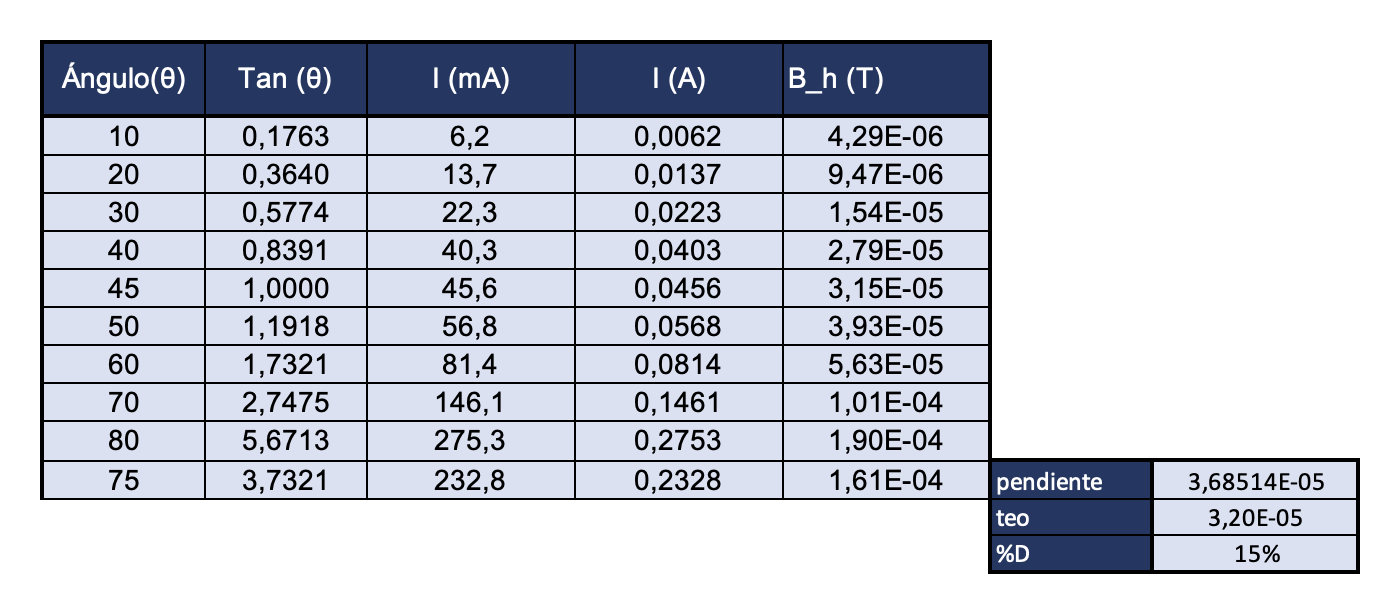
\includegraphics[width=0.8\textwidth]{Figures/1. Content/TablaBHI.png}
        \caption{Tabla de Campo generado por las Bobinas de Helmholtz}
        \label{fig: Tabla de Campo generado por las Bobinas de Helmholtz}
    \end{subfigure}
    \hfill
\end{figure}

\subsection{$B_H$ vs $tan(\Theta)$}
\textbf{Gráfique $B_H$ vs $tan(\Theta)$}

\begin{figure}[H]
  \centering
  \begin{subfigure}[b]{\textwidth}
      \centering
      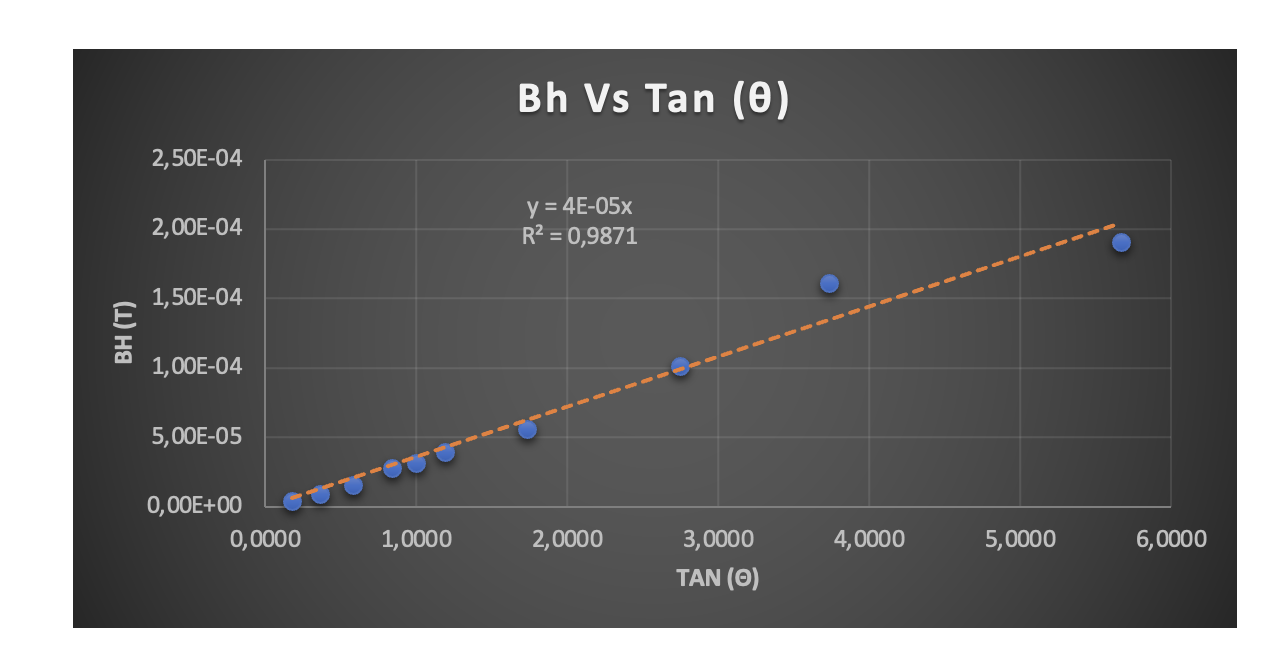
\includegraphics[width=0.8\textwidth]{Figures/1. Content/BHvsTheta.png}
      \caption{$B_H$ vs $tan(\Theta)$}
      \label{fig: B_H vs tanTheta}
  \end{subfigure}
  \hfill
\end{figure}

\subsection{$B_h$ vs $\tan(\theta)$}
\textbf{¿Cómo varía $B_h$ con $\tan(\theta)$?}
El campo magnético $B_h$, medido en teslas, muestra una relación lineal con el $\tan(\theta)$, como se puede observar en la gráfica proporcionada. A medida que aumenta el $\tan(\theta)$, también lo hace el valor de $B_h$, indicando que hay una relación directa entre ambos. La línea de tendencia en la gráfica muestra un ajuste fuerte con un coeficiente de determinación $R^2$ cercano a 1, lo que sugiere una dependencia directa y significativa.

\subsection{Campo magnético terrestre}
\textbf{Encuentre y reporte el campo magnético terrestre haciendo uso de la pendiente de la gráfica anterior (use regresión lineal).}
Utilizando la pendiente de la gráfica, que es $3.68514 \times 10^{-5}$ Tesla, podemos inferir que el campo magnético terrestre en el laboratorio, bajo las condiciones experimentales actuales y suponiendo que la contribución lineal de $\tan(\theta)$ es directamente proporcional al campo terrestre medido, refleja esta pendiente como una medida de cambio en el campo magnético con el ángulo.

\subsection{Error relativo en el campo magnético terrestre}
\textbf{Determine el porcentaje de error relativo si el campo magnético terrestre teórico en el laboratorio es de $3.2 \times 10^{-5}$ T.}
El valor experimental del campo magnético terrestre obtenido fue de $3.68514 \times 10^{-5}$ T. Comparándolo con el valor teórico de $3.2 \times 10^{-5}$ T, el error relativo se calcula como:
\[
\text{Error Relativo} = \left(\frac{|3.68514 \times 10^{-5} - 3.2 \times 10^{-5}|}{3.2 \times 10^{-5}}\right) \times 100\% \approx 15.16\%
\]

\subsection{Factores externos que afectan el cálculo del campo magnético terrestre}
\textbf{¿Qué factores externos pueden afectar el cálculo experimental del campo magnético terrestre en el laboratorio?}
Varios factores externos pueden influir en la medición del campo magnético terrestre en un entorno de laboratorio, incluyendo:
\begin{itemize}
    \item Interferencias electromagnéticas de dispositivos electrónicos cercanos, como computadoras, teléfonos móviles y otros equipos de laboratorio.
    \item Estructuras de metal dentro del edificio que pueden distorsionar o desviar las líneas del campo magnético.
    \item Fluctuaciones temporales en el campo magnético terrestre causadas por cambios atmosféricos o geomagnéticos.
    \item Inexactitudes en el dispositivo de medición, como un teslámetro, especialmente si no está adecuadamente calibrado o es intrínsecamente impreciso a bajas magnitudes de campo magnético.
\end{itemize}


\section{Causas de Error}
Las principales causas de error en este experimento de campos magnéticos podrían incluir:
\begin{itemize}
    \item Errores de calibración en los instrumentos de medición como el teslámetro, que podrían haber afectado las mediciones de campo magnético.
    \item Influencia de objetos metálicos cercanos que podrían distorsionar el campo magnético, especialmente en un entorno de laboratorio donde otros equipos pueden estar presentes.
    \item Fluctuaciones temporales en el campo magnético terrestre, que no se pueden controlar y pueden variar durante el tiempo de medición.
    \item Interferencias electromagnéticas de dispositivos electrónicos cercanos, que pueden alterar significativamente las mediciones del campo magnético.
    \item Inexactitudes en la colocación de los imanes bajo la lámina de vidrio durante el uso de limaduras de hierro, afectando la visualización de las líneas de campo magnético.
\end{itemize}

\section{Conclusiones}
A partir del experimento realizado, se pueden extraer las siguientes conclusiones:
\begin{itemize}
    \item El experimento confirmó visualmente las teorías fundamentales del magnetismo, como la atracción de polos opuestos y la repulsión de polos idénticos, mediante el uso de limaduras de hierro y pruebas de polaridad.
    \item Se logró medir y comparar la fuerza magnética de diferentes tipos de imanes, determinando que la forma y el material del imán afectan significativamente la intensidad del campo magnético generado.
    \item Las mediciones del campo magnético terrestre en el laboratorio mostraron variabilidad y estuvieron sujetas a influencias ambientales y técnicas de medición, destacando la necesidad de un control riguroso del entorno experimental.
    \item El experimento también subrayó la importancia de utilizar instrumentos precisos y bien calibrados para la medición de campos magnéticos, especialmente cuando se comparan con valores teóricos o estándares mundiales como el campo magnético terrestre.
    \item Finalmente, las actividades reforzaron la comprensión práctica de los campos magnéticos y su medición, proporcionando una base sólida para futuras investigaciones o aplicaciones tecnológicas relacionadas con el magnetismo.
\end{itemize}